\section{System Model}
\label{sec:model}

\subsection{The search loop}

\paragraph{Notation.} A collective problem $p$ has a pure-Python
reference $\mathrm{ref}_p(\cdot)$ encoding correctness; a seed
library $\mathcal{S}_p$ of human-written candidate strategies; and
fixed I/O shapes. The search space $\Sigma_p$ is the set of Python
functions with $p$'s signature that compose primitives from the
vendor set
\begin{equation*}
\begin{aligned}
\mathcal{V} \;=\; \{ &\texttt{all\_gather},\; \texttt{reduce\_scatter},\; \texttt{all\_reduce},\\
                     &\texttt{collective\_permute},\; \texttt{all\_to\_all} \,\}
\end{aligned}
\end{equation*}
(all in the \texttt{xm.*} family) together with local XLA ops. A candidate $s \in \Sigma_p$ is admissible if it
matches the reference,
\[
\textsc{Correct}(s) \;=\; \forall \textsc{ws} \in \{4, 8\}:
   \; s(\cdot) = \mathrm{ref}_p(\cdot).
\]
Phase~1 fits a Trainium cost model
$\mathrm{Sim}: \Sigma_p \to \mathbb{R}_{\ge 0}$ from on-device
measurements (Section~\ref{sec:cost}). Phase~4 applies a hardware test that runs the strategy on real
Trainium hardware at the training-shape configuration, returning
$\textsc{Gate}(s) \in \{0, 1\}$ for whether the strategy compiled
and ran without error.
The deployed strategy is
\begin{equation*}
\begin{aligned}
s^\star_p &\;=\; \arg\min_{s \in \Sigma_p^\dagger}\; \mathrm{Sim}(s), \\
\Sigma_p^\dagger &\;=\; \{s \in \Sigma_p : \textsc{Correct}(s) \wedge \textsc{Gate}(s)=1\}.
\end{aligned}
\end{equation*}
The LLM $\mathcal{M}$ acts as a stochastic proposer
$\mathcal{M}: \Sigma_p \to \Sigma_p$ that mutates candidates;
Phase~3 instantiates this as one of three search shapes
(strategy-enumerate / cc-react / multi-island) over a bounded
$\mathcal{M}$-call budget. The five sequential phases that
implement this loop are illustrated in
Figure~\ref{fig:workflow}.

\begin{figure}[t]
\centering
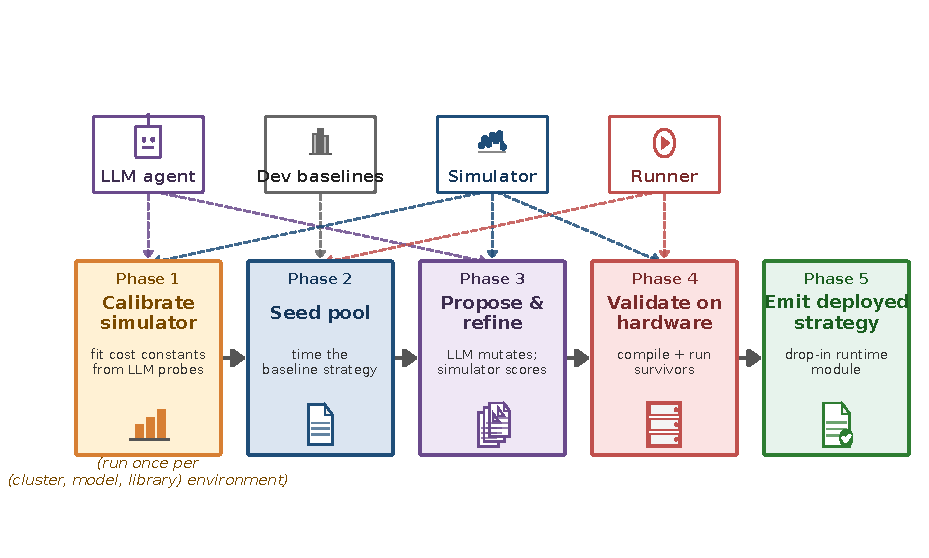
\includegraphics[width=0.95\linewidth]{figures/workflow.pdf}
\caption{Closed-stack search loop. The training workload
supplies tensor shapes and the primitive set. An LLM agent
plays two roles: it writes hardware-specific probing code that
calibrates a workload-faithful cost model on the target device,
and it proposes candidate strategies whose predicted step time
the cost model scores. The top-scoring candidate is validated on
real hardware before being emitted as a drop-in runtime
module. The rest of this section expands the loop into five
sequential phases.}
\label{fig:workflow}
\end{figure}

\paragraph{Phase~1: agent-driven on-device calibration.}
Throughout the paper we refer to the LLM-driven search loop as the
\emph{agent}: a process that proposes, scores, and refines
candidate strategies through several phases. In Phase~1, the
agent is given a set of measurement \emph{tools} (listed in
Table~\ref{tab:probe-tools}) and designs the probe campaign
autonomously: which tensor sizes to sweep, which primitives to
compare, how many repetitions to run, and when to test whether
a measured number really comes from the term it is meant to
isolate (e.g.\ rule out hidden memory-copy overhead by varying
whether the input tensor is stored contiguously in memory). Each tool returns
an empirical scalar or function that wires into one term of
Eq.~\ref{eq:cost}; the agent produces the numerical constants that
populate the simulator. We supply the tools (so the LLM cannot
fabricate numbers), not the experimental design (so the LLM
exploits domain knowledge to choose more informative probes than a
hardcoded script would). Two terms used in the tool list are
worth defining: \emph{EFA} (Elastic Fabric Adapter) is AWS's
RDMA-based cross-node network fabric, used by the cross-node
point-to-point probe; \emph{amortization}, in the back-to-back
tool, refers to the empirical observation that the cost of $k$
consecutive collective calls is typically less than $k$ times
the cost of one call, because the runtime can overlap some of
the per-call overhead across consecutive calls. The tool API
and sweep grids are in Appendix~\ref{sec:profile-impl}.

\begin{table}[!htbp]
\centering\footnotesize
\setlength{\tabcolsep}{3pt}
\setlength{\abovecaptionskip}{2pt}
\setlength{\belowcaptionskip}{0pt}
\begin{tabular}{ll}
\toprule
\textbf{Tool} & \textbf{What it measures} \\
\midrule
\texttt{m\_collective\_lat}   & per-prim latency vs.\ bytes / world size \\
\texttt{m\_p2p\_transfer}     & cross-node point-to-point bandwidth over EFA \\
\texttt{m\_xla\_op\_overhead} & per-op floors for local XLA ops \\
\texttt{m\_compilation\_cost} & cold / cache / reload NEFF compile times \\
\texttt{m\_launch\_overhead}  & per-graph-dispatch (\texttt{mark\_step}) tax \\
\texttt{m\_memcopy\_thru}     & seq.\ and strided host/device copy bw \\
\texttt{m\_b2b\_amortization} & amortization curve for $k$ consecutive collectives \\
\bottomrule
\end{tabular}
\caption{Phase-1 measurement tools the agent is given (prefix
\texttt{m\_} = \texttt{measure\_}). Full identifiers in
Appendix~\ref{sec:profile-impl}.}
\label{tab:probe-tools}
\end{table}

\paragraph{Phase~2: Baseline evaluation.}
A per-problem library of seeded templates is scored through the
simulator. The seed library always contains the
\emph{internal-AWS-optimized baseline} strategy for that
primitive plus a small number of workable but typically naive or
slower alternatives; the per-problem seed lists are given in
Appendix~\ref{sec:phase-code} as code boxes. The baseline we
measure against throughout the paper is the strategy AWS
\emph{uses in production today} to train large-scale MoE and dense
transformer models on Trainium. It is built and confirmed by five
experienced AWS developers who write and maintain Trainium
training paths professionally. The result is the optimized
strategy practitioners actually deploy, not a strawman. The LLM
is not told which seed is the baseline pick. This both calibrates
the simulator's ordering against established practice and seeds
Phase~3.

\paragraph{Phase~3: Agent-driven search.}
The search style we use is \textbf{strategy-enumerate}: the LLM
enumerates $K$ structurally distinct strategies as
natural-language sketches (``pack and gather'', ``per-source
slice loop'', ``masked all-reduce over stacked microbatches'',
$\ldots$), implements each independently, then refines the top-2
by simulator score under a bounded budget
(\S\ref{sec:strat-enum}).

\paragraph{Phase~4: Hardware validation.}
Each Phase-3 survivor runs through a 20-iteration hardware (HW)
microbench plus a 10-step training-validation (TV) harness on a
synthetic 8-layer LM. Crashes, OOMs, NaN at world-scale, or
shape-gate failures exclude the candidate regardless of simulator
score; failed candidates get LLM-assisted recovery (up to two
attempts). HW timing itself is not the ranking signal.

\paragraph{Phase~5: Code generation.}
The lowest \emph{simulator-score} survivor among HW$+$TV passers
wins. We do not pick by HW microbench directly because the
microbench measures isolated-call latency with cached NEFFs and
does not surface the NEFF cache-eviction cost that appears in
real training.

\begin{algorithm}[!htbp]
\caption{End-to-end closed-stack collective-strategy search.}
\label{alg:pipeline}
\begin{algorithmic}[1]
\Require $P$, $\mathrm{ref}(\cdot)$, $\mathcal{S}_P$,
LLM $\mathcal{M}$, profiling tools $\mathcal{T}$, hardware $H$.
\Ensure deployable \texttt{runtime/trainium\_<P>.py}.
\smallskip
\State $\Theta \gets \mathcal{M}.\textsc{calibrate}(\mathcal{T}, H)$
\Comment{Phase~1}
\State $\mathrm{Sim}(\cdot) \gets \textsc{BuildCost}(\Theta)$
\Comment{Eq.~\ref{eq:cost}}
\smallskip
\For{$s \in \mathcal{S}_P$}\Comment{Phase~2}
  \State $\mathrm{score}(s) \gets \mathrm{Sim}(s)$;
  $\textsc{Verify}(s, \mathrm{ref}, \textsc{ws}{\in}\{4,8\})$
  \Comment{verify on small rank counts $\textsc{ws}\!\in\!\{4,8\}$}
\EndFor
\smallskip
\State $\mathcal{C} \gets \textsc{InitPool}(\mathcal{S}_P)$
\Comment{Phase~3 (strategy-enumerate)}
\For{$r = 1 \ldots R$}
  \State $s' \gets \mathcal{M}.\textsc{propose}(\mathcal{C}, \Theta)$
  \If{$\neg\,\textsc{Verify}(s', \mathrm{ref})$} \textbf{continue} \EndIf
  \State $\mathrm{score}(s') \gets \mathrm{Sim}(s')$;
  $\mathcal{C} \gets \mathcal{C} \cup \{s'\}$.
\EndFor
\smallskip
\For{each Phase-3 survivor $s$}\Comment{Phase~4}
  \State $t_{\mathrm{hw}}(s) \gets \textsc{Microbench}(s, H)$
  \State $\textsc{ShapeGate}(s, H)$;
         $\textsc{TVGate}(s, H)$.
  \State $s \gets \mathcal{M}.\textsc{recover}(s)$ \textbf{if}
  gate fails (up to $2\times$).
\EndFor
\smallskip
\State $s^\star \gets \arg\min_{s \in \text{survived}}\,\mathrm{Sim}(s)$
\Comment{Phase~5}
\State $\textsc{Emit}(\texttt{runtime/trainium\_<P>.py},\, s^\star)$;
deploy to $H$.
\end{algorithmic}
\end{algorithm}

\subsection{Cost model}
\label{sec:cost}

The simulator builds a per-step time estimate as the sum of six
physically-grounded terms:
\begin{equation}
\label{eq:cost}
\begin{aligned}
T_{\text{step}} \;=\;
& \underbrace{\textstyle\sum_{i \in \mathcal{L}} c(\mathrm{op}_i, b_i)}_{T_{\text{local}}}
\;+\;
\underbrace{\textstyle\sum_{j} \max(d^{(j)}_{\text{amort}}, b_j / w_{\text{eff}})}_{T_{\text{bw}}} \\
& \;+\;
\underbrace{d_{\text{full}} + (k{-}1)\,d_{\text{amort}}}_{T_{\text{coll}}}
\;+\;
\underbrace{2\,\ell\,m}_{T_{\text{launch}}} \\
& \;+\;
\underbrace{C(b_{\max})\,r/S}_{T_{\text{NEFF}}}
\;+\;
\underbrace{B/w + \pi_{\text{net}}}_{T_{\text{net}}}.
\end{aligned}
\end{equation}
\subsubsection{Per-op local cost ($T_{\text{local}}$).}
$T_{\text{local}}$ sums per-op cost over $\mathcal{L}$, the
chronological list of local XLA ops
the simulator records at trace time. View-only and fused-elementwise
ops pay a small fixed floor; concatenation and stacking
(\texttt{cat}/\texttt{stack}) are bytes-aware, with cost
$\max(\text{floor}, b/w_{\text{seq}})$ where $b$ is bytes moved and
$w_{\text{seq}}$ is the sequential memory bandwidth measured in
Phase~1; contiguity-dependent ops like \texttt{reshape}/\texttt{contiguous}
pay $\max(\text{floor}, b/w_{\text{strided}})$ on non-contiguous
sources, using the lower strided bandwidth measured for non-unit-stride
patterns. This blocks the agent from winning with a chain of
\texttt{narrow}$\to$\texttt{reshape}$\to$\texttt{contiguous} that
looks cheap in isolation but moves the gathered buffer at strided
bandwidth. \texttt{index\_select} and host-side
\texttt{torch.tensor(\ldots)} are volume-scaled by the same rule.
All remaining ops pay their measured isolated cost. Op-category
floors and the \texttt{TrackedTensor} dunder-recording rules are
spelled out in Appendix~\ref{sec:cost-impl-local}.

\subsubsection{Collective bandwidth and back-to-back amortization
($T_{\text{bw}}$, $T_{\text{coll}}$).}
$T_{\text{bw}}$ floors each dispatch at $b_j / w_{\text{eff}}$,
where $w_{\text{eff}}$ comes from the Phase-1 topology object:
cross-node, $w_{\text{eff}}$ is the per-EFA-adapter bandwidth times
the number of adapters per node (Elastic Fabric Adapter, AWS's
high-bandwidth NIC); intra-node it is the per-NeuronLink bandwidth
(NeuronLink is Trainium's on-package interconnect between
NeuronCores). Nothing is hardcoded per problem. $T_{\text{coll}}$
charges $k$ back-to-back dispatches with an amortization schedule
fit empirically: \emph{back-to-back amortization} is the
empirically observed drop in per-call cost when several
collectives fire consecutively inside one launched graph, because
the launch tax and pipeline-fill cost are paid only once. A
shallow chain ($k=1$) pays the full per-call cost; a moderate
chain (a few back-to-back calls) pays a discounted rate as the
network pipeline fills; a deeper chain pays an even lower rate
because the XLA compiler can fuse adjacent collectives into one
NEFF segment. The discount factors are auto-fit from
\texttt{measure\_back\_to\_back\_amortization} probes; the
fitting procedure, converged values on our cluster, and the
run-reset rules that prevent
\texttt{*\,inv}-interleaving from claiming the same amortization
are in Appendix~\ref{sec:cost-impl-coll}.

\subsubsection{Graph-launch and NEFF reload ($T_{\text{launch}}$,
$T_{\text{NEFF}}$, $T_{\text{net}}$).}
$T_{\text{launch}}$ pays $\ell$ from
\texttt{measure\_graph\_launch\_overhead} twice per
\texttt{autograd.Function} boundary (forward \texttt{mark\_step} +
implicit backward \texttt{mark\_step}). The simulator AST-derives
an outer-loop tax that contributes to $m$ in this term; inner
per-tensor/per-bucket loops do not pay it because XLA fuses them
into one NEFF chain. $T_{\text{NEFF}}$ amortizes per-NEFF reload
cost $C(b_{\max})$ over $S$ steps with $r$ reload events under the
default small-cache configuration; $T_{\text{net}}$ adds the
remaining static-byte transfer term. The exact AST rules for
identifying microbatch loops and the per-cluster
\texttt{per\_graph\_neff\_load\_us} default are in
Appendix~\ref{sec:cost-impl-launch}.

\subsubsection{Reward-hacking-resistant structural terms.}
Three structural terms catch HW failure modes that pure-cost
ranking misses.
\begin{enumerate}[leftmargin=*,topsep=2pt,itemsep=2pt]
\item A \textbf{fusion-credit} pass discounts each local compute op
adjacent to a collective with no \texttt{stack}/\texttt{cat}
barrier between them, capturing the compiler-level fusion of
element-wise/reduction ops into a collective's segment.
\item An \textbf{HBM safety} term guards against running out of
high-bandwidth memory (HBM is the per-NeuronCore on-package memory
budget, 16~GB on \texttt{trn1}). Rather than hard-rejecting any
candidate whose peak memory exceeds the budget --- which would let
a single conservative estimate disqualify an otherwise good
strategy --- we apply a smooth quadratic penalty proportional
to how far the estimated peak overruns the budget. A separate
abstract-syntax-tree (AST) pass --- AST is the parsed structure of
the candidate's source code --- recognises explicit byte-budget
assignments (e.g.\ a \texttt{chunk\_size\_bytes = ...} hyperparameter
that bounds a bucketed all-reduce) and propagates that cap into
scaled-byte estimates, so a bucketed algorithm is not charged for
the much-larger flat tensor it would otherwise appear to
materialise.
\item \textbf{Primitive-viability} terms encode two real HW
failure modes: \texttt{xm.collective\_permute} rings at large
world sizes (compiler aborts) and \texttt{xm.all\_reduce} payloads
above the per-collective size limit both receive $+\infty$ cost.
\end{enumerate}
Calibration constants, regex lists, and the world-size failure
pattern are in Appendix~\ref{sec:cost-impl-struct}.

\subsubsection{Phase-5 ranking: why simulator score, not raw
microbench.} Phase~5 ranks survivors by simulator score, not raw
HW microbench latency or TV step time. The HW microbench and the
TV harness are correctness gates: they catch crashes, NaNs, and
shape failures but do not drive ranking. There are two reasons.
First, HW and TV measurements often \emph{fail to generalize to
real multi-rank training}: the microbench runs at small world size
with cached NEFFs and warm caches, the TV harness runs a tiny
8-layer LM that does not exercise the per-step NEFF reload and
back-to-back amortization patterns that dominate at training shape
and 224 ranks --- a strategy that wins at small-scope wall
clock may lose at training scope, and vice versa
(this is the cross-scope-inversion finding the paper documents).
Second, a raw wall-clock number is a sparse reward (no per-op
attribution) that an LLM can game --- stacking metadata-only views
that fuse for free in isolation but force an extra
\texttt{mark\_step} in real training, or moving host-side index
construction into a discarded warmup phase. The simulator
decomposes the reward into per-term contributions with
tool-measured floors, so an optimizer that pushes one term too low
while leaving the others unchanged stops getting credit. The
reward-hacking argument is unpacked as a case study in
Section~\ref{sec:agrs}; the gate fallback rule (when no Phase-3
candidate clears HW+TV gates, deploy the lowest-simulator-score
baseline rather than a sim-only winner that cannot load) is in
Appendix~\ref{sec:cost-impl-phase5}.

\subsection{On-device profiling (Phase~1): the agent builds its
own simulator}
\label{sec:profiling}

The cost model of Section~\ref{sec:cost} is not a fitted
regression nor an offline lookup table: each of its parameters
$\Theta = (\Theta_{\text{net}}, \Theta_{\text{launch}},
\Theta_{\text{NEFF}}, \Theta_{\text{copy}},
\Theta_{\text{neff-cache}})$ is produced by the agent itself,
which calls the probe tools listed in
Table~\ref{tab:probe-tools} on the deployment hardware. In plain
terms: the network parameter $\Theta_{\text{net}}$ is the
straight-line cost model
$T(b,N){=}\alpha(N){+}\beta(N)\,b$ for each collective primitive
at $N$ ranks and $b$ bytes, fit from
\texttt{m\_collective\_lat}; $\Theta_{\text{launch}}$ is the
fixed per-graph-launch overhead measured by
\texttt{m\_launch\_overhead} (about $50$--$200\,\mu$s on
Trainium); $\Theta_{\text{NEFF}}$ summarizes how long it takes
to compile and load a NEFF, measured by
\texttt{m\_compilation\_cost} at four cache tiers (cold compile,
in-process cache, disk NEFF cache, warm re-use) and amortized
across the typical number of steps a NEFF stays resident
($K_{\text{amort}}{\approx}5000$ on our setup);
$\Theta_{\text{copy}}$ is the sequential and strided memcopy
bandwidth from \texttt{m\_memcopy\_thru}; and
$\Theta_{\text{neff-cache}}$ records the back-to-back collective
amortization curve from \texttt{m\_b2b\_amortization} at varying
queue depth.
The exact tool API, sweep grids, and bucket fitting are in
Appendix~\ref{sec:profile-impl}.

Phase~1 calibration takes 8--12 wall-minutes on the 7-node
cluster, runs once per (hardware, software-version) tuple, and
drops its measurements into Eq.~\ref{eq:cost} verbatim. This is
load-bearing: a closed vendor stack updates its collective
implementation, runtime scheduler, and NEFF format across
versions, and the only honest way to track that drift is to
re-measure $\Theta$ against the installed stack rather than
extrapolate from a vendor whitepaper. The ablation in
Section~\ref{sec:ablation-nosim} confirms it: hiding $\Theta$
from the in-loop scoring collapses OLMoE-10B end-to-end from
$1.40\times$ to $1.00\times$ because the LLM-judge falls back to
whichever pattern wins a per-call microbench at small shapes ---
structurally the inline developer baseline. Turning 7-node
microbench per-call latency into a faithful training-step
prediction is what lets the search find strategies whose
per-call latency loses but whose per-step contribution wins (the
AG$+$RS-vs-pack-and-gather case study, Section~\ref{sec:agrs}).

\subsection{Strategy-enumerate loop (Phase~3)}
\label{sec:strat-enum}

Phase~3 takes the Phase-2 seed pool
$\mathcal{S}_P = \{s_0^{(1)}, s_0^{(2)}, \ldots\}$ (the SOTA
developer strategy plus naive or slower alternatives, each
scored by $\mathrm{Sim}(\cdot)$) and runs a bounded LLM-evolution
loop on top. We use an LLM as the mutation oracle here, rather
than classical search methods (e.g.\ random sampling, simulated
annealing, or a genetic algorithm that mutates a fixed grammar
of code templates) because the task is to \emph{author}
candidate code that will be deployed, not to pick a point on a
fixed grammar. Recent work on LLM-driven code synthesis for
performance kernels has established this pattern as
state-of-the-art over rule-, mutation-, and random-search
baselines for compute and communication kernels
\cite{romera2024funsearch, novikov2025alphaevolve,
deepseek2024coder}. The strategy-enumerate variant is a
two-stage layout:

\paragraph{Stage 1: $K$-way strategy enumeration.}
One LLM call enumerates $K$ structurally distinct strategy
sketches
$\{\sigma_1, \ldots, \sigma_K\}$ (we use $K = 5$ throughout the
paper) given:
\begin{enumerate}
  \item the problem's signature
  $\mathrm{sig}_P : \mathcal{X} \to \mathcal{Y}$;
  \item the $\mathcal{S}_P$ reference implementations and their
  simulator scores;
  \item the cost-model parameters
  $\Theta$ flattened into a per-op table.
\end{enumerate}
The LLM emits sketches as
$(\text{name}_k, \text{description}_k)$ pairs; a regex parser
extracts them. Each $\sigma_k$ is then implemented by an
independent second LLM call into runnable Python code
$s_k = \textsc{Impl}(\sigma_k)$, sandbox-executed for correctness
against $\mathrm{ref}(\cdot)$ at world sizes
$\textsc{ws} \in \{4, 8\}$ in 32-bit floating-point precision, and
benchmarked through $\mathrm{Sim}(\cdot)$. We retain $\{s_k\}$ that
pass both correctness and bf16 robustness; up to $K = 5$ candidates
survive.

\paragraph{Stage 2: bounded refinement of the top-2.}
We sort survivors by $\mathrm{Sim}(\cdot)$, take the top two, and
refine each in $R = \lceil \mathrm{maxrounds}/2 \rceil$ rounds
(we use $R = 2$ throughout the paper). Each refinement round
identifies the dominant cost term
$\tau^\star \gets \arg\max_{\tau \in
\{T_{\text{local}}, T_{\text{coll}}, T_{\text{launch}},
T_{\text{NEFF}}, T_{\text{net}}\}} \tau(s)$,
constructs a refine prompt with
$(s, \mathrm{Sim}(s), \tau^\star, \mathrm{breakdown}(s),
\mathrm{history})$, and emits a mutated $s'$. If
$\mathrm{Sim}(s') < \mathrm{Sim}(s)$ and $s'$ passes the
$\mathrm{ref}$+bf16 sandbox, we update $s \gets s'$ and
continue.

Section~\ref{sec:ablation-styles} compares strategy-enumerate
against alternative search styles (a single-trajectory ReAct agent
and a multi-island GA variant) on cost and end-to-end outcome.

\paragraph{Cost calculus vs.\ end-to-end candidate trials.}
Table~\ref{tab:cost-calculus} quantifies the cost advantage of
the loop over the end-to-end-candidate-trial approach (the first
existing option discussed in \S\ref{sec:intro}). The structural
win is that hardware-validation cost is $\mathcal{O}(1)$ per
problem regardless of how many candidate strategies the LLM
explores in Phase~3, whereas the e2e approach pays $\mathcal{O}(K)$
cluster hours for $K$ candidates per problem.

\begin{table}[h]
\centering\scriptsize
\setlength{\tabcolsep}{2.5pt}
\setlength{\abovecaptionskip}{2pt}
\setlength{\belowcaptionskip}{0pt}
\begin{tabular}{@{}p{0.34\columnwidth}p{0.28\columnwidth}p{0.30\columnwidth}@{}}
\toprule
 & \textbf{E2E trials} & \textbf{Our loop} \\
\midrule
Score one candidate           & full training run ($\sim$1\,h) & sim.\ query ($\sim$ms) \\
HW runs / problem             & every candidate                & sim.\ winner only \\
Phase-1 calibration           & N/A                            & $\sim$30\,min cluster \\
LLM cost / problem            & $0$                            & $\sim$\$$2.40$ \\
Scaling in $K$                & $\mathcal{O}(K)$ cluster h     & $\mathcal{O}(1)$ cluster h \\
\midrule
\multicolumn{3}{@{}p{0.95\columnwidth}@{}}{\textit{8 problems, $K{=}5$ per problem, 7-node trn1.32xlarge:}} \\
Cluster time                  & $\sim$$40$\,h                  & $\sim$$8$\,h \\
Cluster cost (\$$150$/h)       & $\sim$\$$6{,}000$              & $\sim$\$$1{,}200{+}$\$$19$\,LLM \\
\bottomrule
\end{tabular}
\caption{Cost calculus, 8-problem suite. The $\sim$5$\times$
saving at $K{=}5$ is a \emph{lower bound}: strategy-enumerate
also scores simulator-refined variants of each candidate for
free, so the effective number of strategies the loop explores
exceeds $K$ while the loop's cluster cost stays $\mathcal{O}(1)$
in the candidate count.}
\label{tab:cost-calculus}
\end{table}

